\documentclass[11pt,a4paper]{article}

% 引入宏包
\usepackage{xeCJK}
\usepackage[margin=0.6in]{geometry} % 极小的页边距，容纳大信息量
\usepackage{hyperref}
\usepackage{enumitem}
\usepackage{titlesec}
\usepackage{xcolor}
\usepackage{graphicx}

% 设置字体 (根据你的系统可更换中文字体，如 SimSun, Microsoft YaHei)
\setCJKmainfont{STSongti-SC-Light} 

% 链接颜色设置 (极客风：深蓝色)
\definecolor{linkblue}{RGB}{0, 50, 150}
\hypersetup{
    colorlinks=true,
    linkcolor=linkblue,
    filecolor=linkblue,      
    urlcolor=linkblue,
    citecolor=linkblue,
}

% 自定义 Section 样式 (带下划线，简洁学术风)
\titleformat{\section}{\large\bfseries\vspace{-0.2em}}{}{0em}{}[\titlerule\vspace{0.2em}]
\titlespacing*{\section}{0pt}{1.2ex plus 1ex minus .2ex}{0.8ex plus .2ex}

% 调整列表间距
\setlist[itemize]{leftmargin=1.5em, nosep, itemsep=0.2em, topsep=0.2em}

% 取消页码
\pagestyle{empty}

\begin{document}

% ==================== 个人信息 ====================
\begin{minipage}[c]{0.78\textwidth}
    {\huge \textbf{孙畅 (Sun Chang)}} \\[0.5em]
    (+86)191-2060-5396 ~|~ \href{mailto:sun.flow@foxmail.com}{sun.flow@foxmail.com}
\end{minipage}
\begin{minipage}[c]{0.2\textwidth}
    \raggedleft
    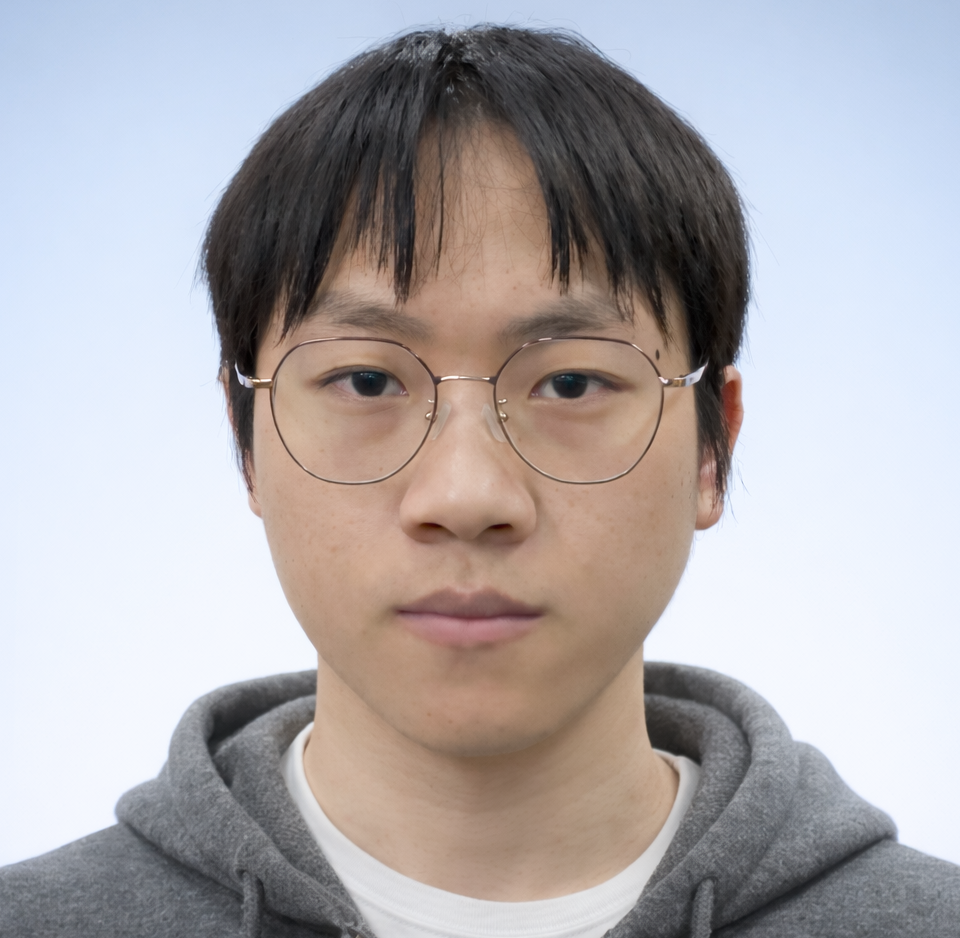
\includegraphics[width=2.5cm]{avatar.png}
    % \framebox[2.5cm]{\rule{0pt}{2cm} \small placeholder}
\end{minipage}

\vspace{-1em}

% ==================== 教育背景 ====================
\section{教育背景}
\noindent
\textbf{华南理工大学} | 电子与信息学院 | 信息与通信工程 | 硕士 \hfill 2024.09—2027.06 (预计)  \\[0.3em]
\noindent
\textbf{华南理工大学} | 物理与光电学院 | 应用物理学 | 学士 \hfill 2020.09—2024.06

% ==================== 专业技能 ====================
\section{专业技能}
\begin{itemize}
    \item 熟悉 Python 及 PyTorch 框架，掌握 Transformers, LLaMA Factory 等大模型开发工具
    \item 深入理解 Transformer 架构, Vision Transformer (ViT), 熟悉 {LLaVA, Qwen-VL} 等多模态架构；精通 {SFT, RLHF, DPO, GRPO} 对齐算法；熟悉 FlashAttention, RoPE, KV-Cache 等底层机制
    \item 掌握基于 token 压缩的模型压缩方法，对大模型轻量化有深入研究
\end{itemize}

% ==================== 项目与工程经历 ====================
\section{项目与工程经历}

% \noindent
% \textbf{从零构建千亿级多模态大模型 (Open-Source Project)} \hfill 开源社区骨干贡献者 \\
% \textit{核心算法开发 / 分布式训练} \hfill 2023.12 -- 至今
% \begin{itemize}
%     \item \textbf{数据清洗与扩展:} 负责 50M 规模的中英文图文对数据清洗，基于 CLIP Score 和自研启发式规则剔除低质量数据，构建高质量预训练语料库。
%     \item \textbf{分布式训练工程:} 基于 \textbf{DeepSpeed ZeRO-3} 和 \textbf{FlashAttention-2} 搭建 64 卡 A100 分布式训练 Pipeline；优化数据加载 Dataloader 解决视觉特征提取的 IO 瓶颈，使总体吞吐量 (TFLOPs) 提升 35\%。
%     \item \textbf{模型对齐 (Alignment):} 主导了模型的 SFT 和 DPO 阶段，通过构造 Hard Negative 多模态偏好数据集，显著降低了模型在图文问答中的拒答率和事实性错误。
% \end{itemize}

% \vspace{0.5em}
% \noindent
% \textbf{大规模视觉语言模型推理加速优化 (实习项目)} \hfill 某一线大厂 AI Lab \\
% \textit{算法工程实习生} \hfill 2023.06 -- 2023.09
% \begin{itemize}
%     \item \textbf{推理引擎集成:} 将自研的 13B MLLM 接入 \textbf{vLLM} 框架，实现 PagedAttention 适配，解决长文本/多图输入时的显存碎片化问题。
%     \item \textbf{量化加速:} 基于 AWQ (Activation-aware Weight Quantization) 算法完成模型的 INT4 量化，精度损失控制在 1\% 以内。
%     \item \textbf{业务落地:} 优化后，模型在单张 RTX 4090 上的首字延迟 (TTFT) 降低 40\%，吞吐量提升 2.5 倍，成功部署于公司的智能客服系统中，日均处理百万级请求。
% \end{itemize}


% ==================== 科研与学术成果 ====================
\section{科研经历与学术成果}
\noindent
\textbf{Streamlined Open-Vocabulary Human-Object Interaction Detection (CVPR 2026)} 第一作者
\begin{itemize}
    \item 基于 DINOv3 架构 VLM 的统一框架 HOI detection
    \item 将 DINOv3 分为前后两部分，利用前一部分特征做细粒度检测，利用后一部分特征做高级语义理解
    \item 用 task-specific query token 连接前后两部分提升对齐质量，同时减少 decode 次数提升模型前向速度
\end{itemize}

\vspace{0.3em}
\noindent
\textbf{Bilateral Collaboration with Large Vision-Language Models for Open Vocabulary Human-Object Interaction Detection (ICCV 2025)} 第三作者
\begin{itemize}
    \item VLM (BLIP-2) 与 DETR 检测模型相互辅助的 HOI detection
    \item 将检测模型得到的 attention map 加到 VLM 的 attention 中，让 VLM 关注到任务需要的细节信息
    \item Detection 与 Next-Token Prediction 任务协同训练，通过梯度反向传播提升模型的整体多模态对齐质量
\end{itemize}

% ==================== 荣誉与奖项 ====================
\section{奖项}
\begin{itemize}
    \item 国家奖学金、学校奖学金
\end{itemize}

\end{document}